% Experimental section for the simulation-grounded LLM traffic optimizer.
% Required packages: \usepackage{amsmath,graphicx}

\section{Experimental Evaluation}
\label{sec:experiments}

We first compare the LLM-feedback optimizer with grounded random search and a
deterministic heuristic under the same microscopic-simulation budget.  We then
reuse the measured LLM candidate pools for an offline Pareto dominance audit.
All aggregates include no-operation outcomes as
zero improvement and therefore evaluate the complete guarded optimizer rather
than only its successful interventions.

\subsection{Experimental Setup}
\label{sec:experimental-setup}

We use five road networks and three demand seeds.  Each frozen demand file was
generated with \texttt{randomTrips.py}~1.24.0 and contains 2,400 passenger trips
departing over one hour.  Baselines and interventions are evaluated with
Eclipse SUMO~1.27.1.  The demand is synthetic and is not calibrated to observed
counts; the experiments therefore test optimization behavior across network
structures rather than real-world traffic fidelity.  Table~\ref{tab:scenario-summary}
summarizes the scenarios.

\begin{table}[!ht]
  \caption{Equal-demand SUMO scenarios. Delay is baseline mean vehicle time
  loss, reported as mean $\pm$ sample standard deviation across three seeds.}
  \label{tab:scenario-summary}
  \begin{center}
    \begin{tabular}{lrrrrr}
      \hline
      City & Edges & Junctions & TLS & Trips & Delay (s) \\
      \hline
      Albany      &  6,193 & 4,309 & 107 & 2,400 & $112.80 \pm 0.26$ \\
      Troy        &  6,107 & 4,355 &  57 & 2,400 & $ 99.79 \pm 0.84$ \\
      Ann Arbor   & 10,151 & 7,522 &  81 & 2,400 & $138.58 \pm 3.13$ \\
      Los Angeles &  6,969 & 4,954 & 172 & 2,400 & $175.76 \pm 1.26$ \\
      Manhattan   &  5,993 & 4,065 & 256 & 2,400 & $245.31 \pm 13.03$ \\
      \hline
    \end{tabular}
  \end{center}
\end{table}

\begin{table}[!ht]
  \caption{Reproducibility settings for the main comparison.}
  \label{tab:reproducibility-settings}
  \begin{center}
    \begin{tabular}{p{0.24\linewidth}p{0.67\linewidth}}
      \hline
      Component & Setting \\
      \hline
      LLM & OpenAI Chat Completions API; \texttt{gpt-5.6-luna}; model-default
      sampling; JSON response mode; 500 output tokens; 60-s timeout and two
      retries after the initial request. \\
      Search budget & At most seven candidate SUMO evaluations per case. LLM
      search uses three grounded initial proposals, up to two feedback
      mutations, and up to two compatible bundles; each baseline uses five
      proposals and up to two bundles. \\
      Candidate space & Signal timing, five-edge corridor speed control,
      single-edge rerouting, and validated topology actions. Numeric choices
      are discrete, and Top-10 ranking excludes edge fragments shorter than
      10~m. \\
      SUMO & Version 1.27.1; 1-s step; complete execution until all vehicles
      arrive; trip-level statistics and emissions plus 60-s edge measurements. \\
      Pairing & For each city and seed, all methods use the same demand, OD
      records, baseline diagnosis, objective, safety constraints, and SUMO
      seed. Only intervention-targeted artifacts are changed. \\
      \hline
    \end{tabular}
  \end{center}
\end{table}

Final selection minimizes time loss on the baseline-frozen Top-10 edges subject
to Equation~\ref{eq:top10-constrained-selection}.  A selected plan must preserve
demand and OD pairs, must not reduce throughput or increase teleports, and may
increase global mean delay and one-hop neighboring time loss by at most 1\% and
5\%, respectively.  The unmodified baseline is always an explicit candidate.

\subsection{Budget-Matched Proposal-Source Comparison}
\label{sec:proposal-source-comparison}

The \emph{LLM feedback} condition begins with one validator-confirmed random
proposal per intervention family.  After SUMO evaluation, the model selects a
single mutation from a finite legal catalog for each retained beam parent.  The
\emph{grounded random} baseline samples supported actions, diagnosed edge and
TLS identifiers, speed factors in $\{0.7,0.8,0.9\}$, and rerouting fractions in
$\{0.25,0.5,0.75,1.0\}$.  The \emph{deterministic heuristic} targets the
highest-ranked bottleneck for corridor and routing actions and the nearest TLS
in the diagnosed subgraph.  The downstream validator, bundle search, simulator,
and selector are shared by all three methods.

In addition to final Top-10 and global-delay reductions, we report proposal
validity and optimization success, defined as selecting a feasible plan with at
least 1\% Top-10 reduction.  Candidate-level simulation efficiency is
\begin{equation}
  \eta_{\mathrm{sim}}=
  \frac{N_{\mathrm{feasible},\,\Delta_{\mathrm{Top10}}\geq1\%}}
       {N_{\mathrm{SUMO}}}.
  \label{eq:simulation-efficiency}
\end{equation}

\IfFileExists{generated/proposal_source_comparison_table.tex}{%
  % Generated by experiment/plot_proposal_source_comparison.py; do not edit by hand.
\begin{table*}[!ht]
  \caption{Budget-matched proposal-source comparison over five networks and three demand seeds. Success denotes a feasible selected plan with at least 1\% Top-10 reduction.}
  \label{tab:proposal-source-comparison}
  \begin{center}
    \small
    \setlength{\tabcolsep}{4pt}
    \resizebox{\textwidth}{!}{%
    \begin{tabular}{lrrrrrr}
      \hline
      Method & Valid (\%) & Success (\%) & Best nets. & Sim. eff. (\%) & Top-10 (\%) & Global (\%) \\
      \hline
      LLM feedback & \textbf{100.0} & \textbf{86.7} & \textbf{3/5} & 35.1 & 9.18 & 2.78 \\
      Grounded random & \textbf{100.0} & 73.3 & 1/5 & 34.0 & 9.00 & \textbf{3.03} \\
      Heuristic & 97.3 & 80.0 & 1/5 & \textbf{39.0} & \textbf{9.60} & 2.69 \\
      \hline
    \end{tabular}
    }
  \end{center}
\end{table*}
%
}{}

\begin{figure*}[!ht]
  \centering
  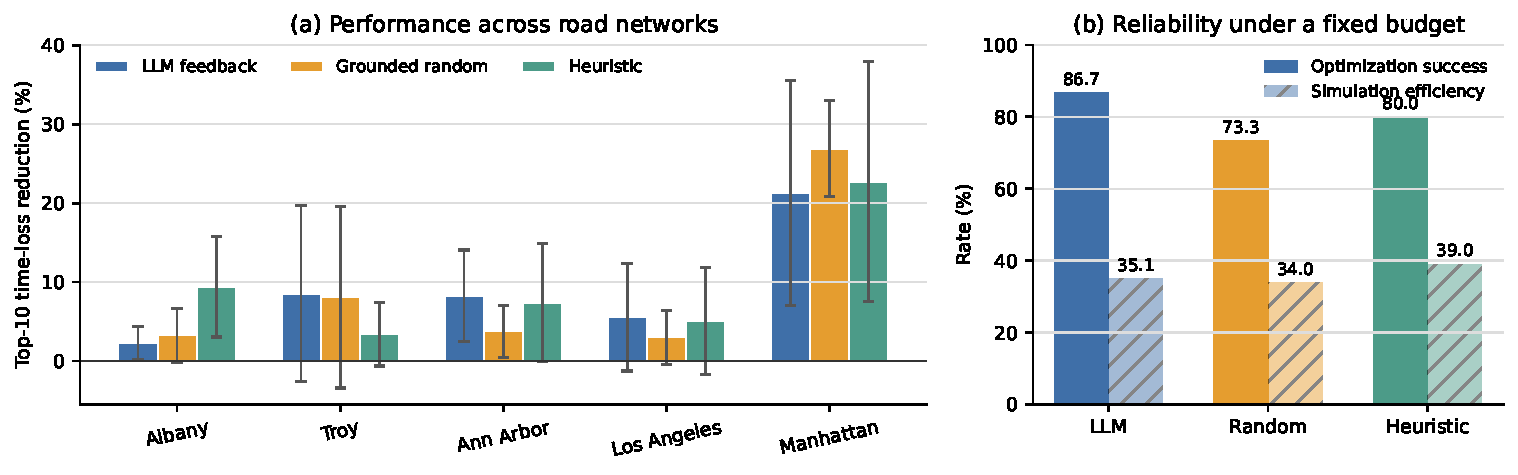
\includegraphics[width=0.96\textwidth]{figures/proposal_source_comparison.pdf}
  \caption{Proposal-source comparison over three demand seeds. Bars in (a)
  show mean Top-10 reduction and sample-standard-deviation error bars. Panel
  (b) reports case-level optimization success and candidate-level simulation
  efficiency under the common seven-evaluation cap.}
  \label{fig:proposal-source-comparison}
\end{figure*}

Across the 15 city--seed cases, LLM feedback attained the highest optimization
success rate (86.7\%) and the lowest no-op rate (13.3\%).  It also achieved the
best seed-averaged Top-10 result in Troy, Ann Arbor, and Los Angeles, whereas
the heuristic led in Albany and grounded random led in Manhattan.  Mean Top-10
reductions were $9.18\%\pm10.18\%$, $9.00\%\pm10.88\%$, and
$9.60\%\pm10.32\%$ for LLM feedback, grounded random, and the heuristic,
respectively.  Their global-delay reductions were 2.78\%, 3.03\%, and 2.69\%.
The LLM's simulation efficiency was 35.1\%, between grounded random (34.0\%)
and the heuristic (39.0\%).  Feedback-refined candidates appeared in seven of
the 15 final LLM plans, showing that measured outcomes changed the search even
though the aggregate advantage was not significant.  Paired Wilcoxon tests on
Top-10 reduction gave $p=0.407$ against random and $p=0.639$ against the
heuristic.  Thus, the evidence supports broader cross-network success rather
than universal superiority over specialized heuristics.

Performance also varies with the demand realization.  Averaged over the five
networks, LLM feedback led seed 42 (12.38\% Top-10 reduction) and seed 44
(10.05\%), whereas the heuristic led seed 43 (9.03\%).  At the paired
city--seed level, LLM feedback beat, tied, and lost to grounded random in six,
six, and three cases, respectively.  It beat the heuristic in six cases and
lost in nine.  The high cross-case standard deviations in
Figure~\ref{fig:proposal-source-comparison} therefore reflect both demand-seed
sensitivity and genuine differences between network structures, particularly
the large attainable improvements in Manhattan.

Table~\ref{tab:five-city-llm-results} reports the proposed optimizer separately
for each network.  Ann Arbor, Los Angeles, and Manhattan accepted a feasible
improving plan for all three demand seeds; Albany and Troy each retained the
baseline once.  Manhattan provides the largest mean reduction and the highest
candidate yield, while the smaller Albany improvements illustrate that the
baseline guard does not force an intervention when the legal search space
offers only marginal or unsafe changes.

\IfFileExists{generated/five_city_llm_results_table.tex}{%
  % Generated by experiment/plot_proposal_source_comparison.py; do not edit by hand.
\begin{table}[!ht]
  \caption{Five-network performance of the LLM-feedback optimizer over three demand seeds. Reductions are mean $\pm$ sample standard deviation in percentage points and include no-op outcomes.}
  \label{tab:five-city-llm-results}
  \begin{center}
    \small
    \setlength{\tabcolsep}{4pt}
    \resizebox{\linewidth}{!}{%
    \begin{tabular}{lrrrr}
      \hline
      Network & Top-10 (\%) & Global delay (\%) & Sim. eff. (\%) & Success \\
      \hline
      Albany & 2.25 $\pm$ 2.11 & 0.17 $\pm$ 0.52 & 21.1 & 2/3 \\
      Troy & 8.55 $\pm$ 11.17 & 0.75 $\pm$ 1.27 & 28.6 & 2/3 \\
      Ann Arbor & 8.25 $\pm$ 5.83 & 1.75 $\pm$ 0.46 & 30.0 & 3/3 \\
      Los Angeles & 5.58 $\pm$ 6.84 & 0.51 $\pm$ 1.28 & 31.6 & 3/3 \\
      Manhattan & 21.27 $\pm$ 14.23 & 10.71 $\pm$ 7.55 & 66.7 & 3/3 \\
      \hline
      Overall & 9.18 $\pm$ 10.18 & 2.78 $\pm$ 5.08 & 35.1 & 13/15 \\
      \hline
    \end{tabular}
    }
  \end{center}
\end{table}
%
}{}

\subsection{Search Behavior and Intervention Composition}
\label{sec:search-behavior}

Figure~\ref{fig:proposal-source-actions} examines how each method reaches its
final decision.  LLM feedback selected five TLS plans, four corridor-speed
plans, four bundles, and two no-ops.  Grounded random selected the same number
of TLS plans and bundles but retained the baseline in four cases, consistent
with its lower optimization-success rate.  The deterministic heuristic was
more concentrated: nine of its 12 applied plans were bundles and the remaining
three used corridor-speed control.  Routing and topology candidates were
evaluated, but none won the final constrained selection because their local
benefits did not compensate for global-delay, spillover, or demand-preservation
failures.

Only three of the 13 applied LLM plans were unmodified initial singles.  Six
were produced by simulation-feedback refinement and four were selected by
bundle search.  Thus, ten applied decisions required a second-stage search
operation rather than merely accepting the grounded random initialization.
This distinction is important because the aggregate comparison otherwise
understates how often measured simulator feedback changes the executable plan.

\begin{figure*}[!ht]
  \centering
  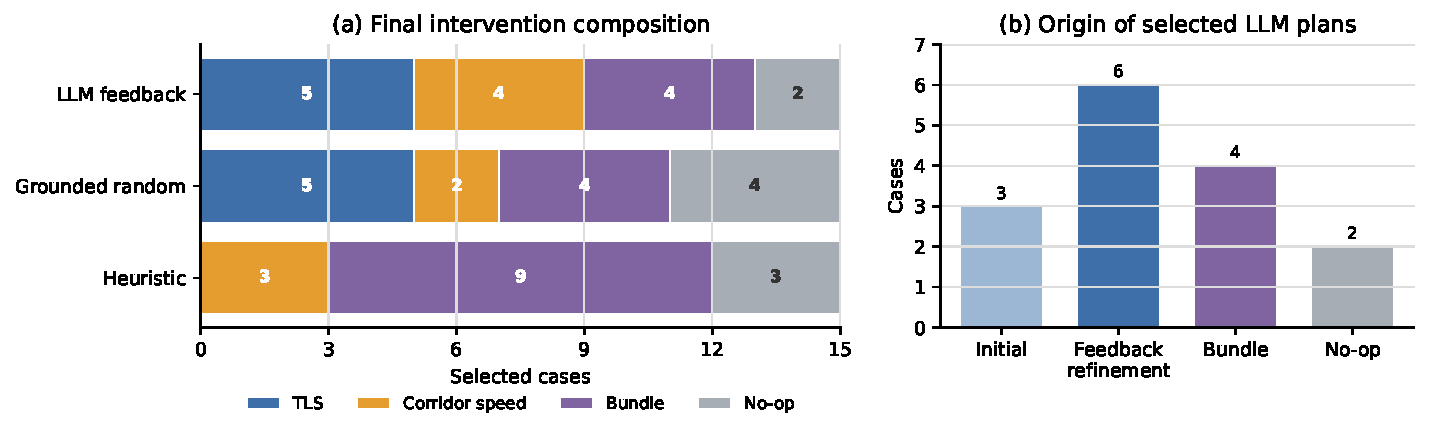
\includegraphics[width=0.92\textwidth]{figures/proposal_source_action_distribution.pdf}
  \caption{Search outcomes over 15 city--seed cases. Panel (a) reports the
  intervention family selected by each proposal source. Panel (b) separates
  initial, feedback-refined, bundled, and no-op outcomes for the LLM search.}
  \label{fig:proposal-source-actions}
\end{figure*}

\subsection{Pareto Dominance Audit}
\label{sec:pareto-results}

We audit the same 15 LLM candidate pools without additional model calls or SUMO
runs.  Dominance is evaluated jointly over Top-10 delay, global delay,
$\mathrm{CO}_2$, and mean speed after applying the operational constraints.
The resulting fronts contain 1.53 candidates on average (range 1--4), and 11 of
the 15 plans selected by the primary Top-10 rule are nondominated.  The four
dominated selections show that optimizing bottleneck delay can sacrifice a
secondary metric, while the generally small fronts indicate limited
multi-objective diversity in the current delay-oriented candidate pools.  We
therefore report Pareto status as a diagnostic rather than introducing
manually weighted profiles or changing the optimizer's primary objective.

\subsection{Threats to Validity}
\label{sec:validity}

Three synthetic demand seeds expose variability but do not provide tight
confidence intervals, and the model-side sampling seed is uncontrolled.  Six
feedback generations failed because of empty or length-limited JSON output;
the LLM therefore used 97 of 105 available evaluations, compared with 103 for
random and 100 for the heuristic.  Simulation efficiency normalizes candidate
yield by realized evaluations, but final-plan quality can still benefit from
greater budget utilization.  Finally, the non-LLM baselines isolate proposal
source within the same action space but are not substitutes for established
traffic-control algorithms or calibrated real-world demand.  We retain all
prompts, structured proposals, validation records, and SUMO outputs for replay.
